%%%%%%%%%%%%%%%%%%%%%%%%%%%%%%%%%%%%%%%%%
% Beamer Presentation
% LaTeX Template
% Version 1.0 (10/11/12)
%
% This template has been downloaded from:
% http://www.LaTeXTemplates.com
%
% License:
% CC BY-NC-SA 3.0 (http://creativecommons.org/licenses/by-nc-sa/3.0/)
%
%%%%%%%%%%%%%%%%%%%%%%%%%%%%%%%%%%%%%%%%%

%----------------------------------------------------------------------------------------
%	PACKAGES AND THEMES
%----------------------------------------------------------------------------------------

\documentclass{beamer}

\mode<presentation> {

% The Beamer class comes with a number of default slide themes
% which change the colors and layouts of slides. Below this is a list
% of all the themes, uncomment each in turn to see what they look like.

%\usetheme{default}
%\usetheme{AnnArbor}
%\usetheme{Antibes}
%\usetheme{Bergen}
%\usetheme{Berkeley}
%\usetheme{Berlin}
%\usetheme{Boadilla}
%\usetheme{CambridgeUS}
%\usetheme{Copenhagen}
%\usetheme{Darmstadt}
%\usetheme{Dresden}
%\usetheme{Frankfurt}
%\usetheme{Goettingen}
%\usetheme{Hannover}
%\usetheme{Ilmenau}
%\usetheme{JuanLesPins}
%\usetheme{Luebeck}
%\usetheme{Madrid}
%\usetheme{Malmoe}
%\usetheme{Marburg}
%\usetheme{Montpellier}
%\usetheme{PaloAlto}
%\usetheme{Pittsburgh}
%\usetheme{Rochester}
\usetheme{Singapore}
%\usetheme{Szeged}
%\usetheme{Warsaw}

% As well as themes, the Beamer class has a number of color themes
% for any slide theme. Uncomment each of these in turn to see how it
% changes the colors of your current slide theme.

%\usecolortheme{albatross}
%\usecolortheme{beaver}
%\usecolortheme{beetle}
%\usecolortheme{crane}
%\usecolortheme{dolphin}
%\usecolortheme{dove}
%\usecolortheme{fly}
%\usecolortheme{lily}
%\usecolortheme{orchid}
%\usecolortheme{rose}
%\usecolortheme{seagull}
%\usecolortheme{seahorse}
%\usecolortheme{whale}
%\usecolortheme{wolverine}

%\setbeamertemplate{footline} % To remove the footer line in all slides uncomment this line
%\setbeamertemplate{footline}[page number] % To replace the footer line in all slides with a simple slide count uncomment this line

%\setbeamertemplate{navigation symbols}{} % To remove the navigation symbols from the bottom of all slides uncomment this line
}
\usepackage{subcaption}
\usepackage[normalem]{ulem}
\usepackage{mathtools}
\usepackage{amsmath}
\usepackage{adjustbox}
\usepackage{graphicx} % Allows including images
\usepackage{booktabs} % Allows the use of \toprule, \midrule and \bottomrule in tables
\usepackage{tikz}
\usepackage[normalem]{ulem}
\usetikzlibrary{arrows,automata}

\graphicspath{{../plots/}}

\newcommand{\com}[1]{}

\newcommand*\pooritem{%
	\item[\color{red}\scalebox{0.9}{\textbullet}]}
\newcommand*\gooditem{%
	\item[\color{blue}\scalebox{0.9}{\textbullet}]}

%\newcommand{\gooditem}[1]{\setbeamercolor{item}{fg=blue}\item #1} 
%\newcommand{\pooritem}[1]{\setbeamercolor{item}{fg=red}\item #1} 
%\setbeamercolor{itemize/enumerate body}{parent=structure}
\DeclarePairedDelimiter\abs{\lvert}{\rvert}%
\DeclarePairedDelimiter\norm{\lVert}{\rVert}%
%----------------------------------------------------------------------------------------
%	TITLE PAGE
%----------------------------------------------------------------------------------------

\title[Conservatism in GEC]{Conservatism and Over-conservatism in Grammatical Error Correction} % The short title appears at the bottom of every slide, the full title is only on the title page

\author{Leshem Choshen \& Omri Abend} 
\institute[Hebrew University Jerusalem Israel] % Your institution as it will appear on the bottom of every slide, may be shorthand to save space
{
Hebrew University Jerusalem Israel\\ % Your institution for the title page
}

\date{July 17 2017} % Date, can be changed to a custom date

\begin{document}

\begin{frame}
\titlepage % Print the title page as the first slide
\end{frame}

%\begin{frame}
%\frametitle{Overview} % Table of contents slide, comment this block out to remove it
%\tableofcontents % Throughout your presentation, if you choose to use \section{} and \subsection{} commands, these will automatically be printed on this slide as an overview of your presentation
%\end{frame}
\AtBeginSection[]
{
	\begin{frame}<beamer>
		\frametitle{Plan}
		\tableofcontents[currentsection]
	\end{frame}
}
%----------------------------------------------------------------------------------------
%	PRESENTATION SLIDES
%----------------------------------------------------------------------------------------
\begin{frame}
	\frametitle{Overview} % Table of contents slide, comment this block out to remove it
	\tableofcontents % Throughout your presentation, if you choose to use \section{} and \subsection{} commands, these will automatically be printed on this slide as an overview of your presentation
\end{frame}

%------------------------------------------------
\section{The task}
\begin{frame}
	\frametitle{\only<2>{\textcolor{green}{T}}\only<1>{t}he task}
	\begin{itemize}

			\item Input: a text which is perhaps \only<1>{ungramatical} \only<2>{\sout{ungramatical}} \only<2>{{\color{green}ungrammatical}}
			\begin{itemize}
				\item Focus learner language (LL)
			\end{itemize}
			\item Output: a grammatical text \only<1>{saying}\only<2>{\sout{saying}} \only<2>{conveying} the same meaning/content.
	\end{itemize}
	\vfill
	\small
	Example:
	However , there are \only<1>{both sides of stories}\only<2>{\sout{both sides of stories}} \only<2>{$\rightarrow$\\
	However , there are \textcolor{green}{two sides to every story.}}

\end{frame}


%------------------------------------------------
\section{Over conservatism}
\begin{frame}
	\frametitle{Conservatism? Over-conservatism?}
	It is a virtue to avoid bad corrections, \\but the goal is still to correct...
	
\end{frame}
\begin{frame}
	\frametitle{Current systems hardly change \emph{sentence boundaries}}
	\begin{figure}
		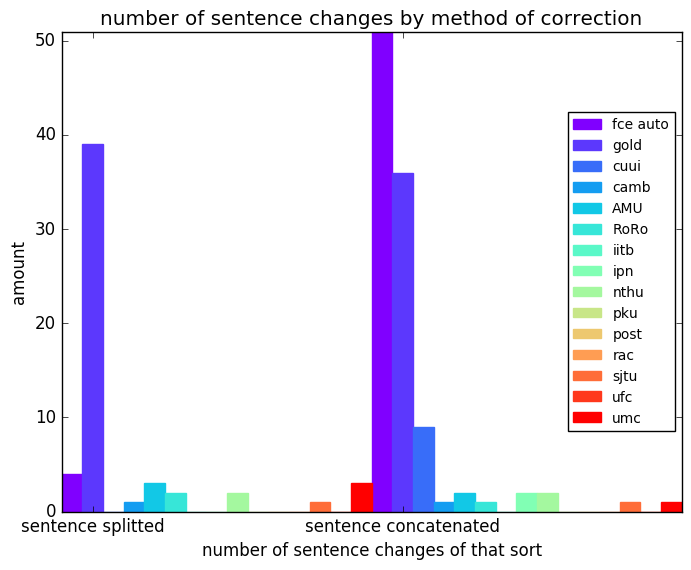
\includegraphics[width = 0.8\textwidth]{aligned}
	\end{figure}
\end{frame}
\begin{frame}
	\frametitle{Current systems hardly change \emph{words}}
	\begin{figure}
		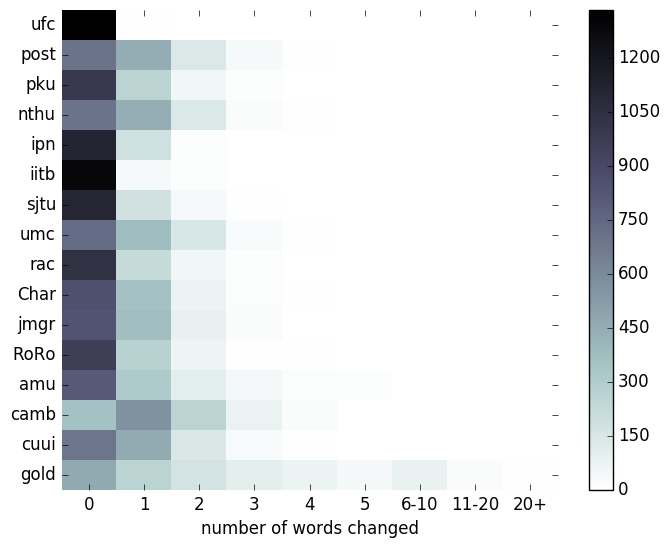
\includegraphics[width = 0.8\textwidth]{words_differences_heat}
	\end{figure}
\end{frame}
\begin{frame}
	\frametitle{Current systems hardly change \emph{word order}}
	\begin{figure}
		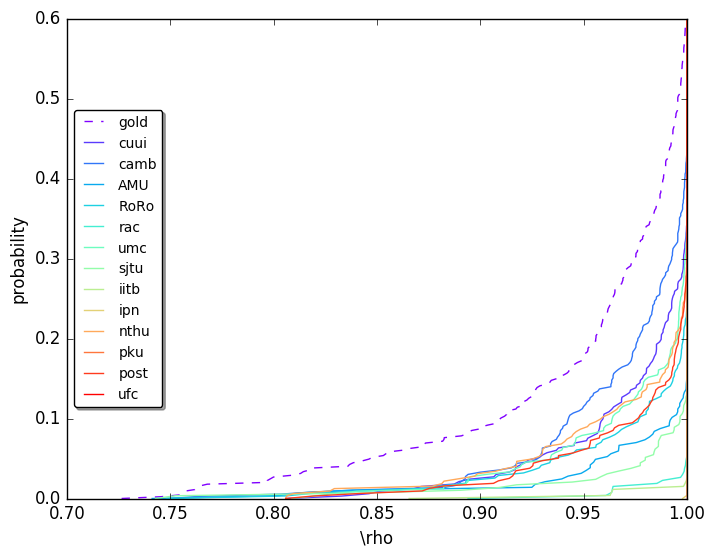
\includegraphics[width = 0.8\textwidth]{spearman_ecdf}
	\end{figure}
\end{frame}
%------------------------------------------------
\section{Reference based measures - (RBM)s}
\subsection{Background and motivation}
\begin{frame}[label=RBM]
	\frametitle{What exists}
	Several Evaluation measures were suggested based on a source and a set of references.\\
	\hyperlink{fscore}{\beamerbutton{$F$-score}}
	\hyperlink{m2}{\beamerbutton{$M^2$}}
	\hyperlink{GLUE}{\beamerbutton{GLUE}}
	\hyperlink{I-measure}{\beamerbutton{I-measure}}\\
	To Train and validate 1 reference per source sentence.
\end{frame}

\begin{frame}
	\frametitle{Corrections as distribution}
	\begin{itemize}
		\item Each sentence $x$ has a set of valid corrections $correct_x$
		\item $\mathcal{D}_x$ a distribution of human corrections
		\item For testing - $Y\sim \mathcal{D}_x^M$ a sample of $M$ references 
		\item $P_{coverage}$ - $P_{y\sim \mathcal{D}_x}(y \in Y)$
	\end{itemize}
\end{frame}

\begin{frame}
	\frametitle{Analytical worries}
	If a system detected a mistake it is incentivized to correct if 
	$$p_{correct} \cdot p_{coverage} > 1-p_{detect} $$
	If there is $\alpha$ punishment for wrong corrections
	$$p_{correct} \cdot p_{coverage} - \left(1-p_{correct}\cdot p_{coverage}\right) \alpha > 1-p_{detect}$$
\end{frame}
\begin{frame}
	\frametitle{Empirical confirmation}
	\begin{figure}
		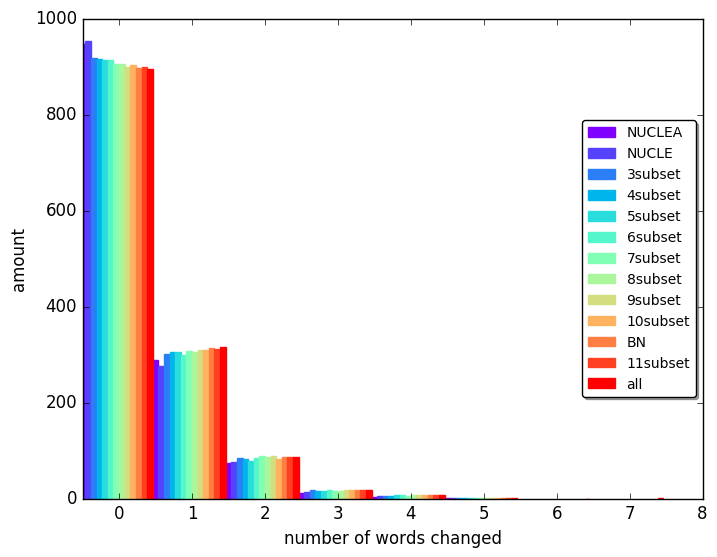
\includegraphics[width=8cm]{words_differences_hist_reranking}
	\end{figure}
\end{frame}

\subsection{Corrections as distribution}
\begin{frame}
	\frametitle{Estimating $\mathcal{D}$}
	To estimate $\mathcal{D}$ we use UnseenEst.
	It estimates the histogram minimizing earthmover distance.
\end{frame}
\begin{frame}[label=Dists]
	\frametitle{Findings}
	\begin{table}[h!]
		\begin{tabular}{c|c|c|c|c|}
			%\cline{2-5} 
			& \multicolumn{4}{c|}{Frequency Threshold ($\gamma$)}\\ 
			%\cline{2-5} 
			& \multicolumn{1}{c}{0} & \multicolumn{1}{c}{0.001} & \multicolumn{1}{c}{0.01} & \multicolumn{1}{c|}{0.1}
			\\
			\hline
			Variants & 1351.24 & 74.34 & 8.72 & 1.35
			\\
			Mass & 1 & 0.75 & 0.58 & 0.37\\
			\hline
		\end{tabular}
	\end{table}\hyperlink{alldists}{\beamerbutton{dists}}
\end{frame}
\begin{frame}
	\frametitle{Yet more findings}
	\framesubtitle{Rare corrections still count}
	\begin{figure}
		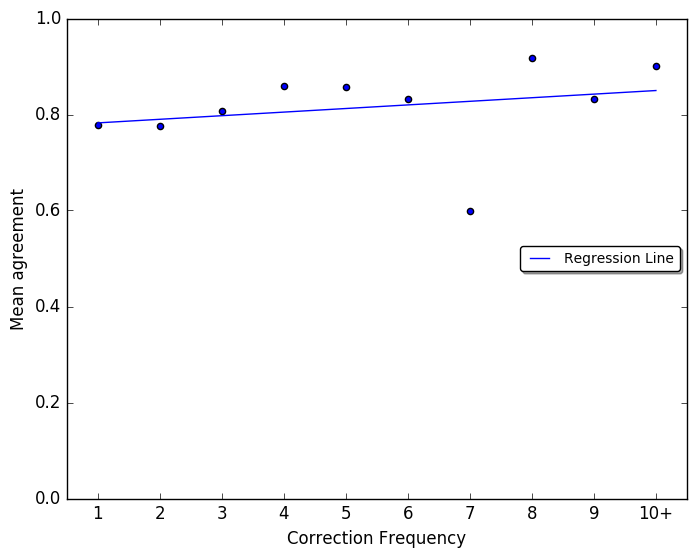
\includegraphics[width=8cm]{IAA_confirmation_frequency}
	\end{figure}
\end{frame}
\subsection{RBMs under estimation as a function of $M$}
\begin{frame}
	\frametitle{Accuracy - analysis}
	Given a perfect corrector, how well will it do?
	$\frac{1}{N}\sum_{i=1}^N P_{Y \sim \mathcal{D}_i^M, y \sim \mathcal{D}_i}\left(y \in Y\right)$
	\begin{figure}
		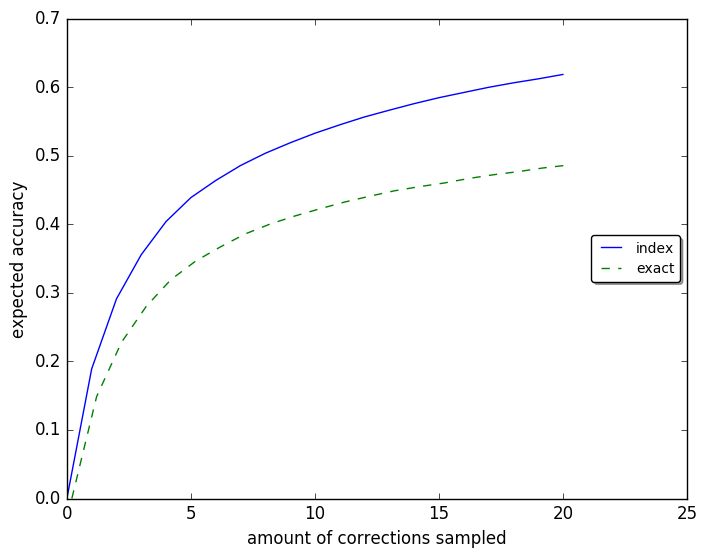
\includegraphics[width=8cm]{noSig_repeat_1000_accuracy}
	\end{figure}
\end{frame}
\begin{frame}
	\frametitle{$F$-score - empirical}
		\begin{figure}
			\includegraphics[width=8cm]{$F_{0.5}$_Ms_significance}
		\end{figure}
	Note: with repetition it is more or less the same
\end{frame}
\begin{frame}
	\frametitle{Significance}
	human vs. machine

	\begin{figure}
		\includegraphics[width=8cm]{$F_{0.5}$_significance}
	\end{figure}
\end{frame}
\section{Reference-less semantic measure}
\begin{frame}
	\frametitle{Reference-less evaluation}
	Input: Corrected sentences and Source sentences \sout{and references in the form of sentences}.
	
	Output: A score, but which?!
\end{frame}
\begin{frame}
	\frametitle{Reference-less evaluation}
	Compare the source and the reference
	\begin{itemize}
		\gooditem Suggestion: compare grammar annotations
		\pooritem Grammar is ill defined with ungrammatical text
		\pooritem Some define grammar on ungrammatical text as reference some as source
	\end{itemize}
\end{frame}
\begin{frame}
	\frametitle{Reference-less evaluation}
	Combine two measures (worked for MT)
	\begin{enumerate}
		\item faithfulness -- semantic similarity of the correction and the source. \footnote{\tiny Leshem Choshen and Omri Abend. "Conservatism and Over-conservatism in Grammatical Error Correction" - this work}
		\item grammaticality -- error detection over the source \footnote{\tiny Napoles Courtney, Keisuke Sakaguchi, and Joel Tetreault. "There's No Comparison: Reference-less Evaluation Metrics in Grammatical Error Correction." arXiv preprint arXiv:1610.02124 (2016).}
	\end{enumerate}
\end{frame}

\begin{frame}
	\frametitle{UCCA}
	\begin{itemize}
		\item Semantic annotation scheme that builds on
		typological and cognitive linguistic theories
		\item Provides a coarse-grained, cross-linguistically
		applicable representation
		\item Structures are DAGS, words are leaves
		\item Text is a collection of {\it Scenes} and relations between them
	\end{itemize}
\end{frame}
\begin{frame}[label=distances-details]
	\frametitle{Measures}
	\begin{itemize}
		\item IAA - percentage of Nodes with same label and leaves
		\item UCCASim - percentage of Nodes with same label and most matched leaves
		\item Top down - size of the biggest cut
		\item Token - Consider only main entities
		\item (Labeled) Tree edit - tree distance when ordered by tokens alignment 
	\end{itemize}
	\hyperlink{distances}{\beamerbutton{distances table}}
\end{frame}

\begin{frame}[label=UCCA]
	\frametitle{LL hypotheses}
	\begin{itemize}
		\item LL can be annotated using UCCA
		\item Corrections change grammar, not semantics
	\end{itemize}
	\hyperlink{annotated}{\beamerbutton{all annotation}}
\end{frame}

\begin{frame}
	\frametitle{Corrections preserve meaning}
	\begin{table}
		\begin{tabular}{c|c|c|c||c|c|}
			\cline{2-6} 
			& \multicolumn{3}{c||}{\sc UCCASim} & \multicolumn{2}{c|}{\sc DistSim}\\ \cline{2-6}
			& s$\rightarrow$r & r$\rightarrow$s & Avg & A+D & Scene\
			\\
			\hline
			Different & 0.85 & 0.83 & 0.84 & 0.96 & 0.93
			\\
			Same & 0.92 & 0.91 & 0.92 & 0.97 & 0.96
			\\
			\hline
			\hline
			IAA & 0.85 & 0.81 & 0.83 & - & -
			\\
			\hline
			SAR15 & - & - & - & 0.95 & 0.96 \\
			\hline
		\end{tabular}
	\end{table}
\end{frame}

\begin{frame}
	\frametitle{Works also automatically (TUPA parser)}
	\begin{table}
		\begin{tabular}{c|c|c|c|}
			\cline{2-4} 
			& \multicolumn{3}{c|}{\sc UCCASim} \\
			\cline{2-4}
			& s$\rightarrow$r & r$\rightarrow$s & Avg\
			\\
			\hline
			TUPA & 0.7 & 0.7 & 0.7
			\\
			\hline
			\hline
			Different & 0.85 & 0.83 & 0.84
			\\
			\hline
		\end{tabular}
	\end{table}
\end{frame}

\begin{frame}
	\Huge{\centerline{Any more questions?}}
\end{frame}


\appendix
%------------------------------------------------
\section{Motivations}
\begin{frame}
	\frametitle{Motivation - Natural Language Processing view}
		Spelling correction is a solved problem, this is the next step.
		\uncover<2->{
		\begin{figure}
		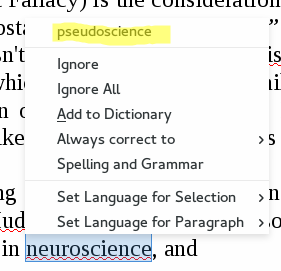
\includegraphics[width=0.5\linewidth]{unnamed}
		\end{figure}}
\end{frame}

\begin{frame}
	\frametitle{Motivation - Practice}
	English is a second language for the majority of English speakers.
	
	It can be used to enhance learning, as a tool (e.g. the green line in Word) etc.

\end{frame}

\begin{frame}
	\frametitle{Motivation - Computational Linguistics}
	Understanding grammatical errors and the way they can be corrected may lead to better understanding of innate processes and language behaviour.
	\begin{itemize}
		\item what errors do people do? why?
		\item what do we need to know in order to correct a language?
		\item what mistakes people will never do?
		\item Does learners' languages differ from native languages? 
	\end{itemize}
\end{frame}
\section{Data}
\begin{frame}
	\frametitle{What data is there?}
	Field research and linguistic evidence
	
	Two types of corpora:
	\begin{itemize}
		\item native or learner language corpora
		\begin{itemize}
			\item large 
			\item cheap 
		\end{itemize}
		\item parallel corpora
		\begin{itemize}
			\item both learner language and their corrections \item corrections tend to be in the form of edits
		\end{itemize}
	\end{itemize}
\end{frame}
%------------------------------------------------
%%%%%%%%%%% outline
\section{Grammatical error correction approaches}
\subsection{Classifier}
\begin{frame}
	\frametitle{Classifier based}
	\begin{itemize}
		\item Different types of errors are chosen (e.g. Noun number errors)
		\item For each a set of possible corrections are chosen (e.g. $\{s,\emptyset\}$)
		\item A Classifier is built for each error type
		\item These are combined with rule based components (e.g. add e before the s when...)
	\end{itemize}
\begin{figure}
		\centering
		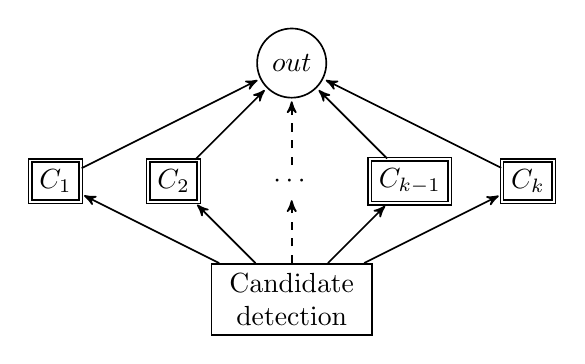
\begin{tikzpicture}[->,>=stealth', shorten >=1pt, auto, node distance=1.5cm, semithick]
		\node[draw, text width = 1.8cm, align = center] (A)                    {Candidate detection};
		\node[dashed,double] (B) [above of=A] {$\cdots$};
		\node[state] (output) [above of=B] {$out$};
		\node[draw,double] (C) [left of=B] 		{$C_2$};
		\node[draw,double] (D) [left of=C]  		{$C_1$};
		\node[draw,double] (E) [right of=B]  		{$C_{k-1}$};
		\node[draw,double] (F) [right of=E]  		{$C_k$};
		\path
		(B) edge[dashed] (output)
		(C) edge (output)
		(D) edge (output)
		(E) edge (output)
		(F) edge (output)
		(A) edge[dashed] (B)
		(A) edge (C)
		(A) edge (D)
		(A) edge (E)
		(A) edge (F);
		
		\end{tikzpicture}
	\end{figure}
\end{frame}
\begin{frame}
	\frametitle{Classifier based - pro con}
	\begin{itemize}
		\pooritem Can only correct the chosen errors
		\pooritem Complex mistakes and interleaving mistakes can not be handled properly
		\gooditem Can generalize to similar problems with unseen words
		\gooditem Useful in an unsupervised scenario
	\end{itemize}
\end{frame}
\subsection{Machine Translation}
\begin{frame}
\frametitle{Machine Translation - motivation}
A learner language is a consistent language, we can learn how to translate from it to the proper language.
\end{frame}

\begin{frame}
	\frametitle{Machine Translation - main idea}
	The main idea behind MT is the noisy channel.
	\centering
	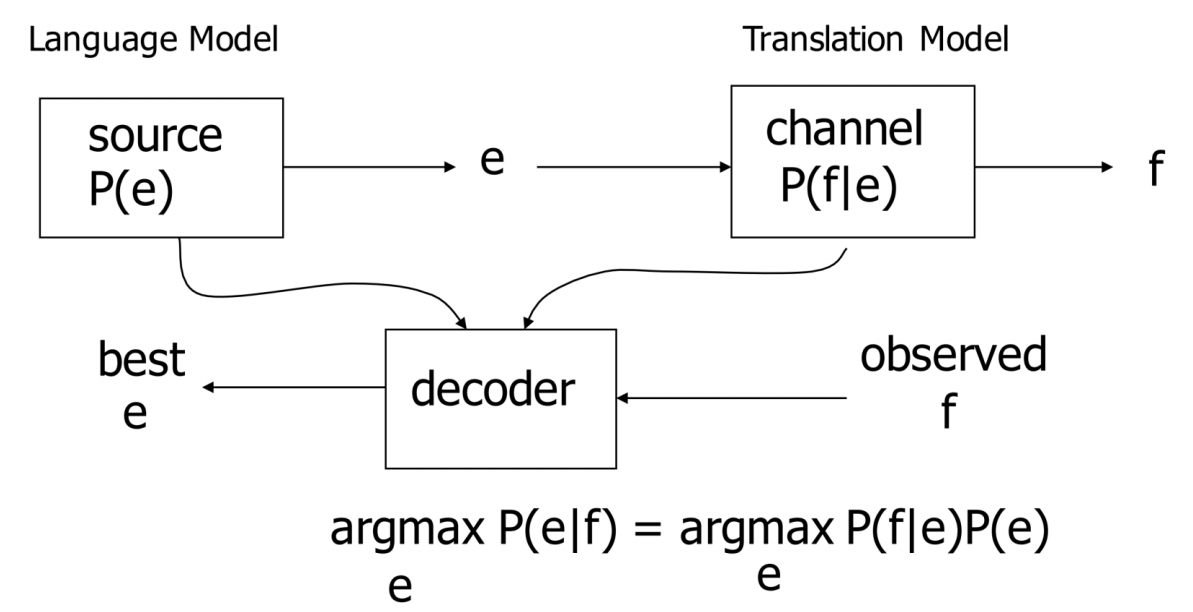
\includegraphics[width=0.8\linewidth]{noisy}
\end{frame}

\begin{frame}
	\frametitle{Machine Translation - components}
	Language model -- a model assigning a probability for a sentence to appear in the language $p\left(e\right)$
	
	Translation model -- uses a parallel corpus to assign probabilities to $p\left(f|e\right)$ 
	\begin{figure}
		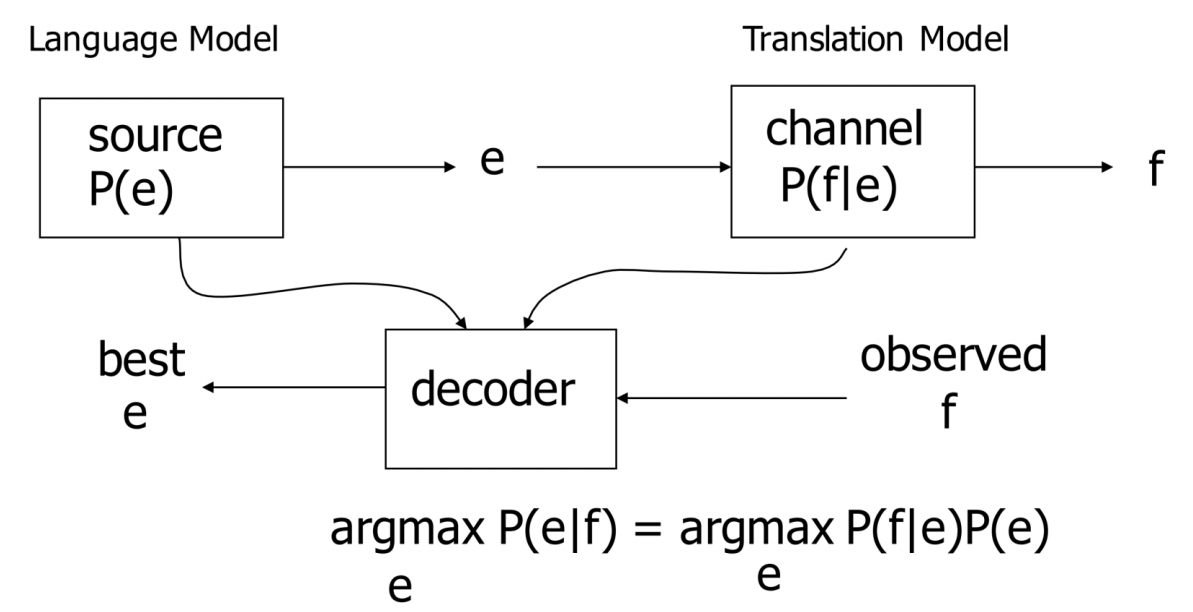
\includegraphics[width=0.8\linewidth]{noisy}
	\end{figure}
\end{frame}

\begin{frame}
	\frametitle{And (of course) Neural Networks}
	Standard neural machine translation methods has started to immigrate to grammatical error correction too.\footnote{\tiny Chollampatt, Shamil, Kaveh Taghipour, and Hwee Tou Ng. "Neural network translation models for grammatical error correction." arXiv preprint arXiv:1606.00189 (2016).}\footnote{\tiny Yuan, Zheng, and Ted Briscoe. "Grammatical error correction using neural machine translation." Proceedings of NAACL-HLT. 2016.}
	\begin{figure}[b]
		\centering
			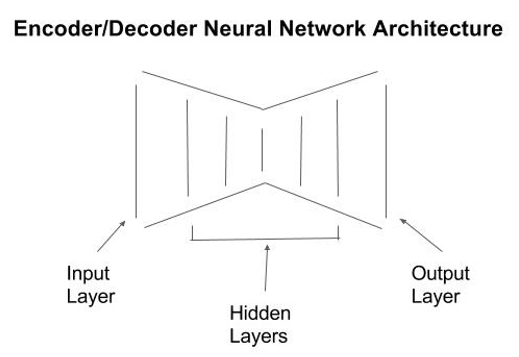
\includegraphics[width=.6\linewidth]{encdec}
	\end{figure}
\end{frame}

\begin{frame}
	\frametitle{MT - pro con}
	\begin{itemize}
		\gooditem Can correct the various errors
		\gooditem Complex mistakes and interleaving mistakes can be handled properly
		\pooritem Have problems generalizing to similar problems with unseen words (or phrases)
		\pooritem Less useful in an unsupervised scenario
	\end{itemize}
\end{frame}

\begin{frame}
	\frametitle{hybrid}
	Overall MT is good for many errors but the classifiers are better on the specific classes of errors chosen.
	
	A pipeline starting with classifiers and applying MT over the results.
	This approach was shown to get the benefits of both models.\footnote{\tiny Alla Rozovskaya, and Dan Roth. "Grammatical error correction: Machine translation and classifiers." Urbana 51 (2016): 61820.}
\end{frame}

%------------------------------------------------
\section{Evaluation}
\subsection{Naive}
\begin{frame}[label=fscore]
	\frametitle{Edit $F$-score}
	Input: Corrected phrase-edits, references in the form of gold phrase edits.\footnote{\tiny Dale, Robert, and Adam Kilgarriff. "Helping our own: The HOO 2011 pilot shared task." Proceedings of the 13th European Workshop on Natural Language Generation. Association for Computational Linguistics, 2011.}
	
	Output: phrase edit $F$-score 
	\small Back to \hyperlink{RBM}{\beamerbutton{RBMs}}.
\end{frame}

\begin{frame}
	\frametitle{Phrase edits $F$-score}
	\centering
	\uncover<1>{A correction is True iff the same \emph{edit} is found in a reference.
		
		For each sentence the best matching reference is used.
	}
	\uncover<2>{
		No-correction should be preferred over wrong correction,\\ thus $F_{0.5}$,  emphasizing precision, is used
		$$F_\beta = (1 + \beta^2) \cdot \frac{\mathrm{precision} \cdot \mathrm{recall}}{(\beta^2 \cdot \mathrm{precision}) + \mathrm{recall}}$$}
	\begin{figure}[b]
		\centering
		\begin{subfigure}{.3\textwidth}
			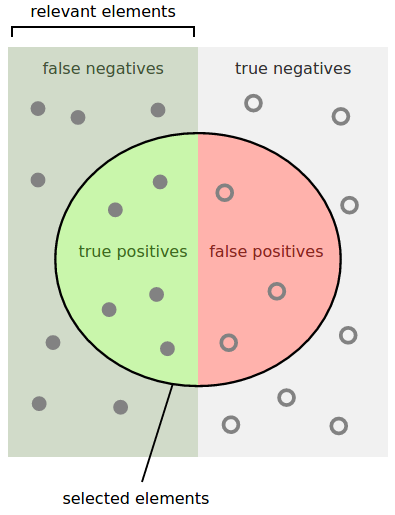
\includegraphics[width=\linewidth]{TP_TN}
		\end{subfigure}%
		\begin{subfigure}{.5\textwidth}
			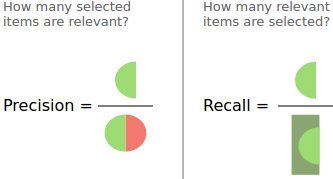
\includegraphics[width=\linewidth]{P_R}
		\end{subfigure}
	\end{figure}
	\small Back to \hyperlink{RBM}{\beamerbutton{RBMs}}.
\end{frame}

\begin{frame}
	\frametitle{Edit $F$-score}
	But we do not expect correctors to actually mark what was the edit. Especially not in the same way humans ``do".
	
	\small \{a $\rightarrow \emptyset$ \} or \{a words $\rightarrow words$\}
	\small Back to \hyperlink{RBM}{\beamerbutton{RBMs}}.
\end{frame}

\subsection{$M^2$-scorer}
\begin{frame}[label=m2]
	\frametitle{$M^2$-scorer}
	Input: Corrected sentences, Source sentences and references in the form of gold phrase edits.\footnote{\tiny Dahlmeier, Daniel, and Hwee Tou Ng. "Better evaluation for grammatical error correction." Proceedings of the 2012 Conference of the North American Chapter of the Association for Computational Linguistics: Human Language Technologies. Association for Computational Linguistics, 2012.}
	
	Output: phrase edit $F$-score
	\small Back to \hyperlink{RBM}{\beamerbutton{RBMs}}.
\end{frame}

\begin{frame}
	\frametitle{$M^2$-scorer -- corrections are sentences, not edits}
	An up to $n$ words edit distance is computed dynamically, and a lattice is made. A negative value is assigned to every edit that is shown in the reference.
	\begin{figure}[b]
		\centering
		\begin{subfigure}{.8\textwidth}
			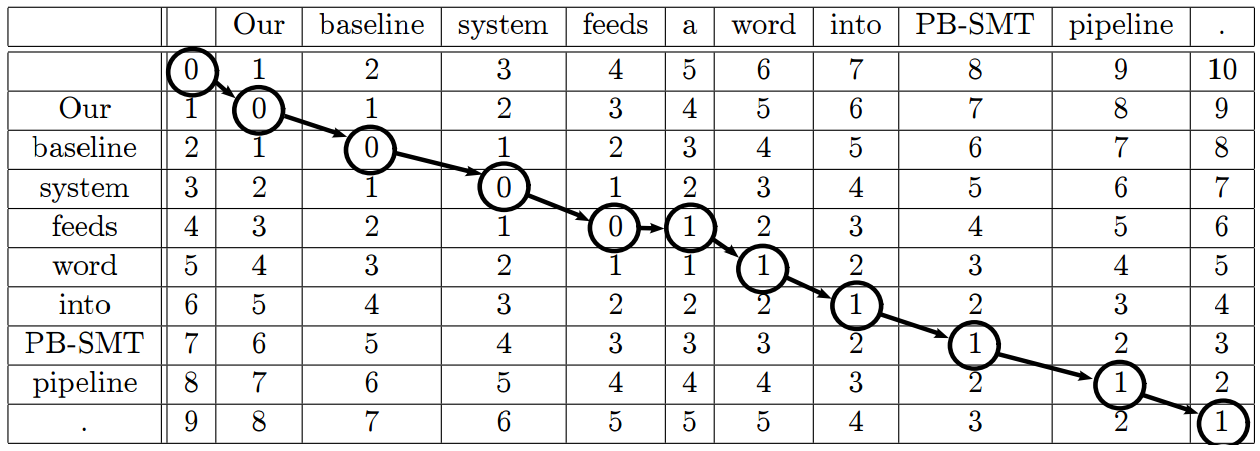
\includegraphics[width=\linewidth]{lattice}
		\end{subfigure}
		
		\begin{subfigure}{\textwidth}
			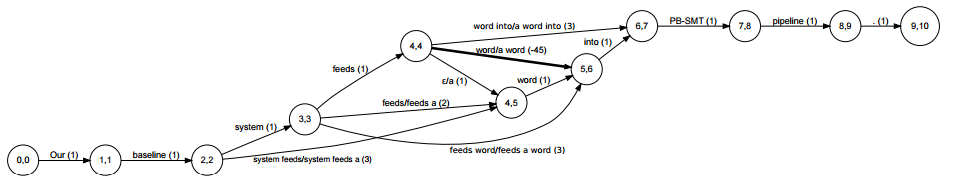
\includegraphics[width=\linewidth]{paths}
		\end{subfigure}
	\end{figure}
	\small Back to \hyperlink{RBM}{\beamerbutton{RBMs}}.
\end{frame}
\subsection{I-measure}
\begin{frame}
	\frametitle{I-measure}
		Input: Corrected sentences, Source sentences and references in the form of gold word edits.\footnote{\tiny Felice, Mariano, and Ted Briscoe. "Towards a standard evaluation method for grammatical error detection and correction." HLT-NAACL. 2015.}
		
		Output: Token-level weighted accuracy
	\small Back to \hyperlink{RBM}{\beamerbutton{RBMs}}.
\end{frame}

% show all alerts and only open solutions one by one
%\begin{frame}
%	\frametitle{I-measure}
%	\begin{itemize}[<+(1)->]
%		\item <alert@*> {\color{red}Phrase edit choices are prone to errors}
%		\item {\color{blue}Use correction-source-reference word alignment maximizing Sum of Pairs}
%		\item <alert@*> {\color{red}$F$-score ignores TN (choices not to correct)}
%		\item {\color{blue}Use accuracy}
%		\item <alert@*> {\color{red}Wrong corrections and no correction is the same for accuracy}
%		\item {\color{blue}Weighting is introduced}
%	\end{itemize}
%	$$W_{acc}=\frac{w\cdot TP + TN}{w\cdot\left(TP+TN\right) TN + FN - \left(w+1\right)\cdot\frac{FPN \footnote{places where correction source and reference all differ}}{2}}$$
%\end{frame}

\begin{frame}[label=I-measure]
	\frametitle{I-measure}
	\begin{itemize}[<+->]
		\pooritem {\color{red}Phrase edit choices are prone to errors (partial match, lack of TN count)}
		\gooditem {\color{blue}Use correction-source-reference word alignment maximizing Sum of Pairs}
		\pooritem {\color{red}$F$-score ignores TN (choices not to correct)}
		\gooditem {\color{blue}Use accuracy}
		\pooritem {\color{red}Wrong corrections and no correction is the same for accuracy.}
		\gooditem {\color{blue}Weighting is introduced}
		\gooditem {\color{blue} Comparison with the source is made possible.}
	\end{itemize}
	$$W_{acc}=\frac{w\cdot TP + TN}{w\cdot\left(TP+TN\right) TN + FN - \left(w+1\right)\cdot\frac{FPN \footnote{places where correction, source and reference all differ}}{2}}$$
	\small Back to \hyperlink{RBM}{\beamerbutton{RBMs}}.
\end{frame}

\subsection{GLEU}
\begin{frame}[label=GLUE]
	\frametitle{GLEU}
		Input: Corrected sentences, Source sentences and references in the form of sentences. \footnote{\tiny Napoles, Courtney, et al. "Ground truth for grammatical error correction metrics." Proceedings of the 53rd Annual Meeting of the Association for Computational Linguistics and the 7th International Joint Conference on Natural Language Processing. Vol. 2. 2015.}
		
		Output: Weighted precision of n-gram (BLEU-like)
		\small Back to \hyperlink{RBM}{\beamerbutton{RBMs}}.
\end{frame}
\begin{frame}
	\frametitle{GLEU - details}
	\begin{itemize}
		\pooritem \color{red} Without weights the source has the second best score
		\gooditem \color{blue} Extra weight to valid corrections (overlap with R not S)
		\item Penalty for no correction (overlap with S not R)
	\end{itemize}
	\small Back to \hyperlink{RBM}{\beamerbutton{RBMs}}.
\end{frame}
\begin{frame}
	\frametitle{GLEU - Human Rankings}
	Shown to achieve higher correlation with humans.
	\begin{figure}[b]
		\centering
		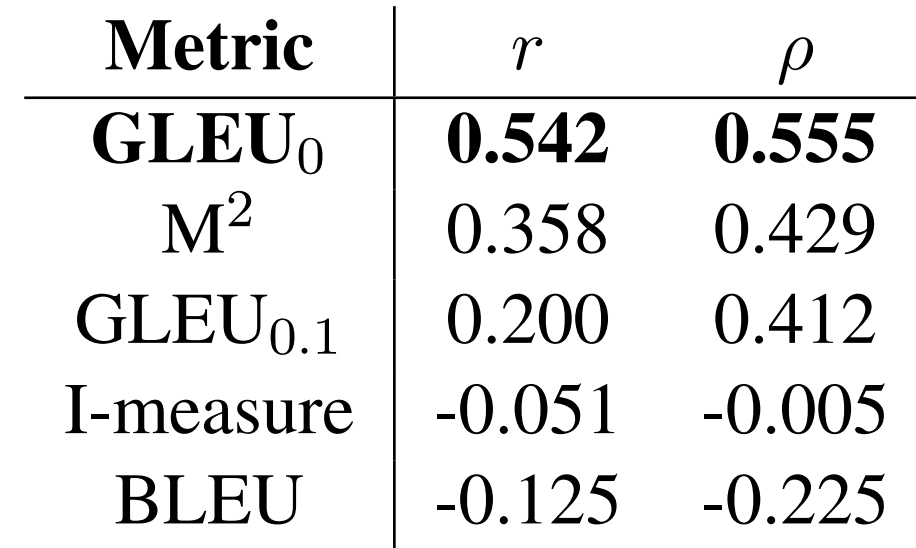
\includegraphics[width=.6\linewidth]{humanJudge}
	\end{figure}
	\small Back to \hyperlink{RBM}{\beamerbutton{RBMs}}.
\end{frame}

\subsection{reference-less}
\begin{frame}
	\frametitle{Findings}
	Only a handful of references are used, While even a short sentence tends to have hundreds of different valid corrections. It leads to under estimations.
	\begin{figure}[b]
		\centering
		\includegraphics[width=.6\linewidth]{$F_{0.5}$_Ms_significance}
		\caption{$M^2$ scores of a perfect corrector by the number of references}
	\end{figure}
\end{frame}

\begin{frame}[label=distances]
	\begin{table}[]
		\centering
		\footnotesize
		\begin{tabular}{l|l|l|l|l|l|l|}
			&                                    &                              &                               & \multicolumn{3}{c|}{Token}                                                          \\ \cline{2-7} 
			& \multicolumn{1}{c|}{Tree} & \multicolumn{1}{c|}{UCCASim} & \multicolumn{1}{c|}{Top down} & \multicolumn{1}{c|}{Bottom up} & \multicolumn{1}{c|}{Top down} & \multicolumn{1}{c|}{UCCASim} \\ \cline{2-7} 
			Different                 & 324.57                             & 0.83                         & 0.75                          & 0.74                           & 0.72                          & 0.83                         \\
			Same                      & 211.50                             & 0.88                         & 0.85                          & 0.83                           & 0.79                          & 0.88                         \\ \hline
			\multicolumn{1}{|l|}{IAA} & 285.69                             & 0.88                         & 0.78                          & 0.80                           & 0.75                          & 0.87                         \\ \hline
		\end{tabular}
	\end{table}
	\small Back to \hyperlink{distances-details}{\beamerbutton{details}}.
\end{frame}

\begin{frame}[label=annotated]
\begin{table}[]
	\centering
	\scriptsize
	\begin{tabular}{lll}
		Annotator-id & NUCLE-id & type      \\
		1         & 2  & corrected \\
		2         & 2  & corrected \\
		1         & 2  & learner   \\
		2         & 2  & learner   \\
		1         & 3  & corrected \\
		2         & 3  & corrected \\
		1         & 3  & learner   \\
		2         & 3  & learner   \\
		1         & 5  & corrected \\
		2         & 5  & corrected \\
		1         & 5  & learner   \\
		2         & 5  & learner   \\
		1         & 6  & learner   \\
		2         & 6  & learner   \\
		2         & 7  & corrected \\
		2         & 7  & learner   \\
		1         & 8  & corrected \\
		1         & 8  & learner   \\
		1         & 10 & corrected \\
		1         & 10 & learner  
	\end{tabular}
\end{table}
\small Back to \hyperlink{UCCA}{\beamerbutton{UCCA}}.
\end{frame}
\begin{frame}[label=alldists]
	\frametitle{Distributions}
	\begin{figure}
		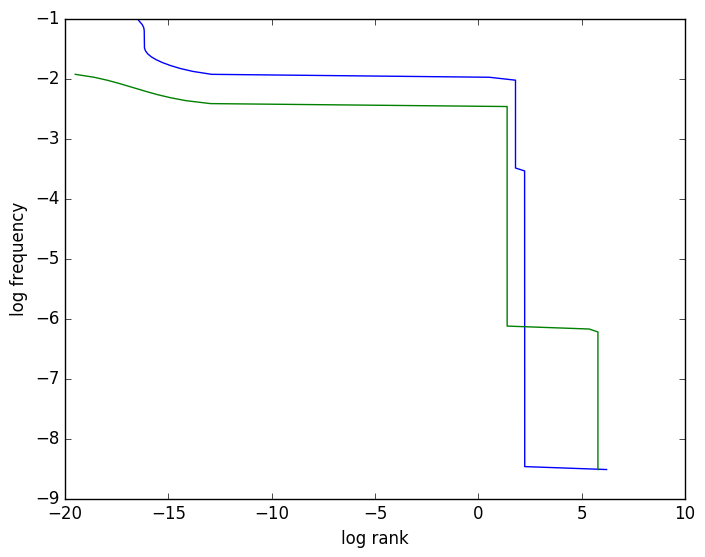
\includegraphics[width=8cm]{exact_dists_plot}
	\end{figure}
		\small Back to \hyperlink{Dists}{\beamerbutton{Dists}}
\end{frame}
\begin{frame}
	\frametitle{Distributions}
	\small Back to \hyperlink{Dists}{\beamerbutton{Dists}}
	\begin{figure}
		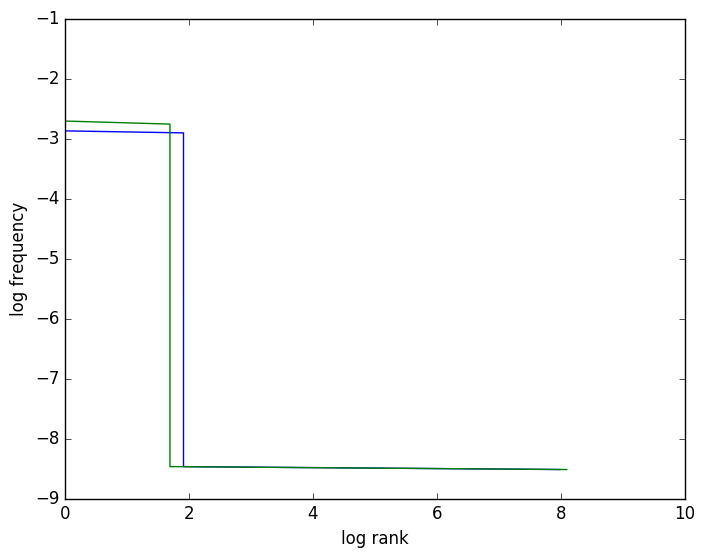
\includegraphics[width=8cm]{2_random_exact_dists_plot}
	\end{figure}
\end{frame}
\end{document} 